\documentclass{article}
\usepackage{graphicx} % Required for inserting images
\usepackage[absolute,overlay]{textpos}
\setlength{\parindent}{0pt}
\usepackage{geometry}
\geometry{top=1in, bottom=1in, right=1in, left=1in}
\usepackage{multicol}
\usepackage{multirow}
\usepackage[pages=some]{background}

\pagestyle{empty}

\backgroundsetup{
  scale=1,
  opacity=1,
  angle=0,
  contents={
\includegraphics[width=\paperwidth,height=\paperheight]{imagenes/portada.jpg}}
}

\usepackage{xcolor}
\definecolor{rojo}{rgb}{0.8, 0, 0}

\usepackage{titlesec}


\titleformat{\section}
  {\color{rojo}\Large\bfseries}
  {}
  {0pt}
  {}

\titleformat{\subsection}
  {\color{rojo}\large\bfseries}
  {}
  {0pt}
  {}

\begin{document}
\BgThispage
\-
\begin{textblock*}{15cm}(4cm, 9cm)
    {\fontsize{30pt}{16pt}\selectfont
    \textcolor{rojo}{\textbf{REPORTE DE PRÁCTICA NO. ?}}
    }
\end{textblock*}
\begin{textblock*}{15cm}(4cm, 11cm)
    {\fontsize{15pt}{16pt}\selectfont
    \textcolor{rojo}{\textbf{NOMBRE DE LA PRÁCTICA}}
    }
\end{textblock*}
\begin{textblock*}{15cm}(4cm, 12cm)
    {\fontsize{13pt}{16pt}\selectfont
    \textcolor{rojo}{\textbf{ALUMNO:}}
    }
\end{textblock*}
\begin{textblock*}{15cm}(6cm, 12.5cm)
  {\fontsize{11pt}{16pt}\selectfont
  	extcolor{rojo}{\textbf{Rogelio Rocha Hernandez}}
  }
\end{textblock*}

\newpage

\section{1. Alfabeto}

Un alfabeto (representado por la letra griega $\Sigma$) es un conjunto finito y no vacío de símbolos que sirven como base para construir cadenas o palabras.
Estos símbolos pueden ser letras, números o cualquier carácter definido por el contexto del lenguaje formal.
El alfabeto es el punto de partida para definir un lenguaje, ya que todos los elementos de éste deben formarse exclusivamente con los símbolos que lo integran.

\paragraph{Ejemplos:}

$\Sigma = \{0,1\}$ \(\to\) Alfabeto binario utilizado en sistemas digitales.

$\Sigma = \{a, b, c\}$ \(\to\) Alfabeto de tres símbolos común en ejemplos teóricos.

\section{2. Cadenas}

Una cadena o palabra es una secuencia finita de símbolos que pertenecen al alfabeto.
La longitud de una cadena se expresa por el número de símbolos que contiene.
Las cadenas son los elementos básicos con los que se forman los lenguajes.

\paragraph{Ejemplos:}

Si $\Sigma = \{a, b\}$, entonces ``abba'' es una cadena válida.

Si $\Sigma = \{0, 1\}$, entonces ``1010'' pertenece al lenguaje binario.

\section{3. Cadena Vacía}

La cadena vacía, representada por $\varepsilon$, es una cadena especial que no contiene ningún símbolo y cuya longitud es cero.
Aunque parece no tener valor, cumple un papel importante en la teoría de lenguajes, ya que se considera parte de cualquier lenguaje formal.

La cadena vacía no debe confundirse con un espacio en blanco, ya que representa la ausencia total de caracteres.

\paragraph{Ejemplo:}

En el lenguaje $L = \{\varepsilon, a, ab\}$, la cadena vacía $\varepsilon$ forma parte del conjunto.

\section{4. Propiedades de las Palabras}

Las propiedades de las palabras permiten analizar su estructura interna y definir relaciones entre cadenas.
Las más relevantes son:

\begin{itemize}
  \item Longitud: número de símbolos que contiene una cadena.
  \item Prefijo: parte inicial de una palabra.
  \item Sufijo: parte final de una palabra.
  \item Subcadena: secuencia de símbolos contenida dentro de otra cadena.
  \item Concatenación: unión de dos cadenas de manera secuencial.
\end{itemize}

\section{5. Combinaciones (Concatenación)}

La concatenación es una operación fundamental que une dos cadenas de forma consecutiva para formar una nueva.
Si se tienen dos cadenas $x$ e $y$, su concatenación se denota como $xy$.
Esta operación no es conmutativa, es decir, $xy \neq yx$ en la mayoría de los casos.

\paragraph{Ejemplo:}

Si x = \texttt{ab} y y = \texttt{c}, entonces \texttt{xy} = \texttt{abc} y \texttt{yx} = \texttt{cab}.

Si x = \texttt{10} y y = \texttt{01}, entonces \texttt{xy} = \texttt{1001}.

\section{6. Clausura de Kleene ($\Sigma^*$)}

La Clausura de Kleene es una operación que genera todas las posibles cadenas (incluyendo la vacía) que pueden formarse con los símbolos de un alfabeto.
Formalmente, se define como:
$\Sigma^* = \{\varepsilon\} \cup \Sigma \cup \Sigma^2 \cup \Sigma^3 \cup \dots$

Es un concepto esencial en la construcción de lenguajes formales, ya que permite representar la totalidad de las combinaciones posibles de un alfabeto dado.

\paragraph{Ejemplo:}
Si $\Sigma = \{a, b\}$, entonces:
$\Sigma^* = \{\varepsilon, a, b, aa, ab, ba, bb, aaa, aab, \dots\}$

\section{7. Autómatas}

Un autómata es un modelo matemático que simula el comportamiento de una máquina que procesa símbolos de entrada y decide si la cadena es aceptada o rechazada, según un conjunto de reglas o transiciones.
El estudio de los autómatas es fundamental en la teoría de la computación, ya que permite modelar y analizar el funcionamiento de programas, compiladores y lenguajes.

\paragraph{Ejemplo:}
Un autómata puede aceptar solo cadenas que terminen en ``1'':

Entrada: ``101'' \(\to\) Aceptada

Entrada: ``100'' \(\to\) Rechazada

\section{8. Tipos de Autómatas y Usos}

Los autómatas se clasifican según su complejidad y capacidad de reconocimiento:

\begin{table}[!ht]
\centering
\begin{tabular}{|l|l|l|}
\hline
Tipo de Autómata & Descripción & Aplicación \\
\hline
Autómata Finito Determinista (AFD) & Cada estado tiene una única transición para cada símbolo. & Verificación de contraseñas o validación de secuencias. \\
\hline
Autómata Finito No Determinista (AFND) & Puede haber múltiples transiciones posibles para un símbolo. & Procesamiento de expresiones regulares. \\
\hline
Autómata con Pila (AP) & Utiliza una pila para recordar símbolos. & Análisis de estructuras anidadas (como paréntesis). \\
\hline
Máquina de Turing (MT) & Modelo más general que representa cualquier algoritmo. & Estudio teórico de la computación y programación. \\
\hline
\end{tabular}
\caption{Tipos de autómatas y sus usos}
\end{table}

\paragraph{Ejemplo:}
Un autómata con pila puede verificar si los paréntesis en una expresión están balanceados:


  exttt{(()())} \(\to\) Correcto

  exttt{(()} \(\to\) Incorrecto

\section{}

Los conceptos de alfabeto, cadenas, propiedades, clausura de Kleene y autómatas son pilares de la teoría de los lenguajes formales.
Estos elementos permiten construir modelos abstractos que representan procesos lógicos y computacionales, esenciales para el desarrollo de compiladores, validadores de sintaxis, y sistemas automáticos de reconocimiento de patrones.

El entendimiento de estos temas facilita el análisis de cómo los lenguajes son interpretados y procesados por las máquinas, sentando las bases de la teoría de la computación y el diseño de software inteligente.

\newpage
\newpage

\begin{figure}[!ht]
  \centering
  \begin{minipage}{0.48\textwidth}
    \centering
    
\includegraphics[width=0.9\linewidth]{imagenes/Imagen de WhatsApp 2025-10-17 a las 07.08.08_2f0da4f9.jpg}
  \end{minipage}\hfill
  \begin{minipage}{0.48\textwidth}
    \centering
    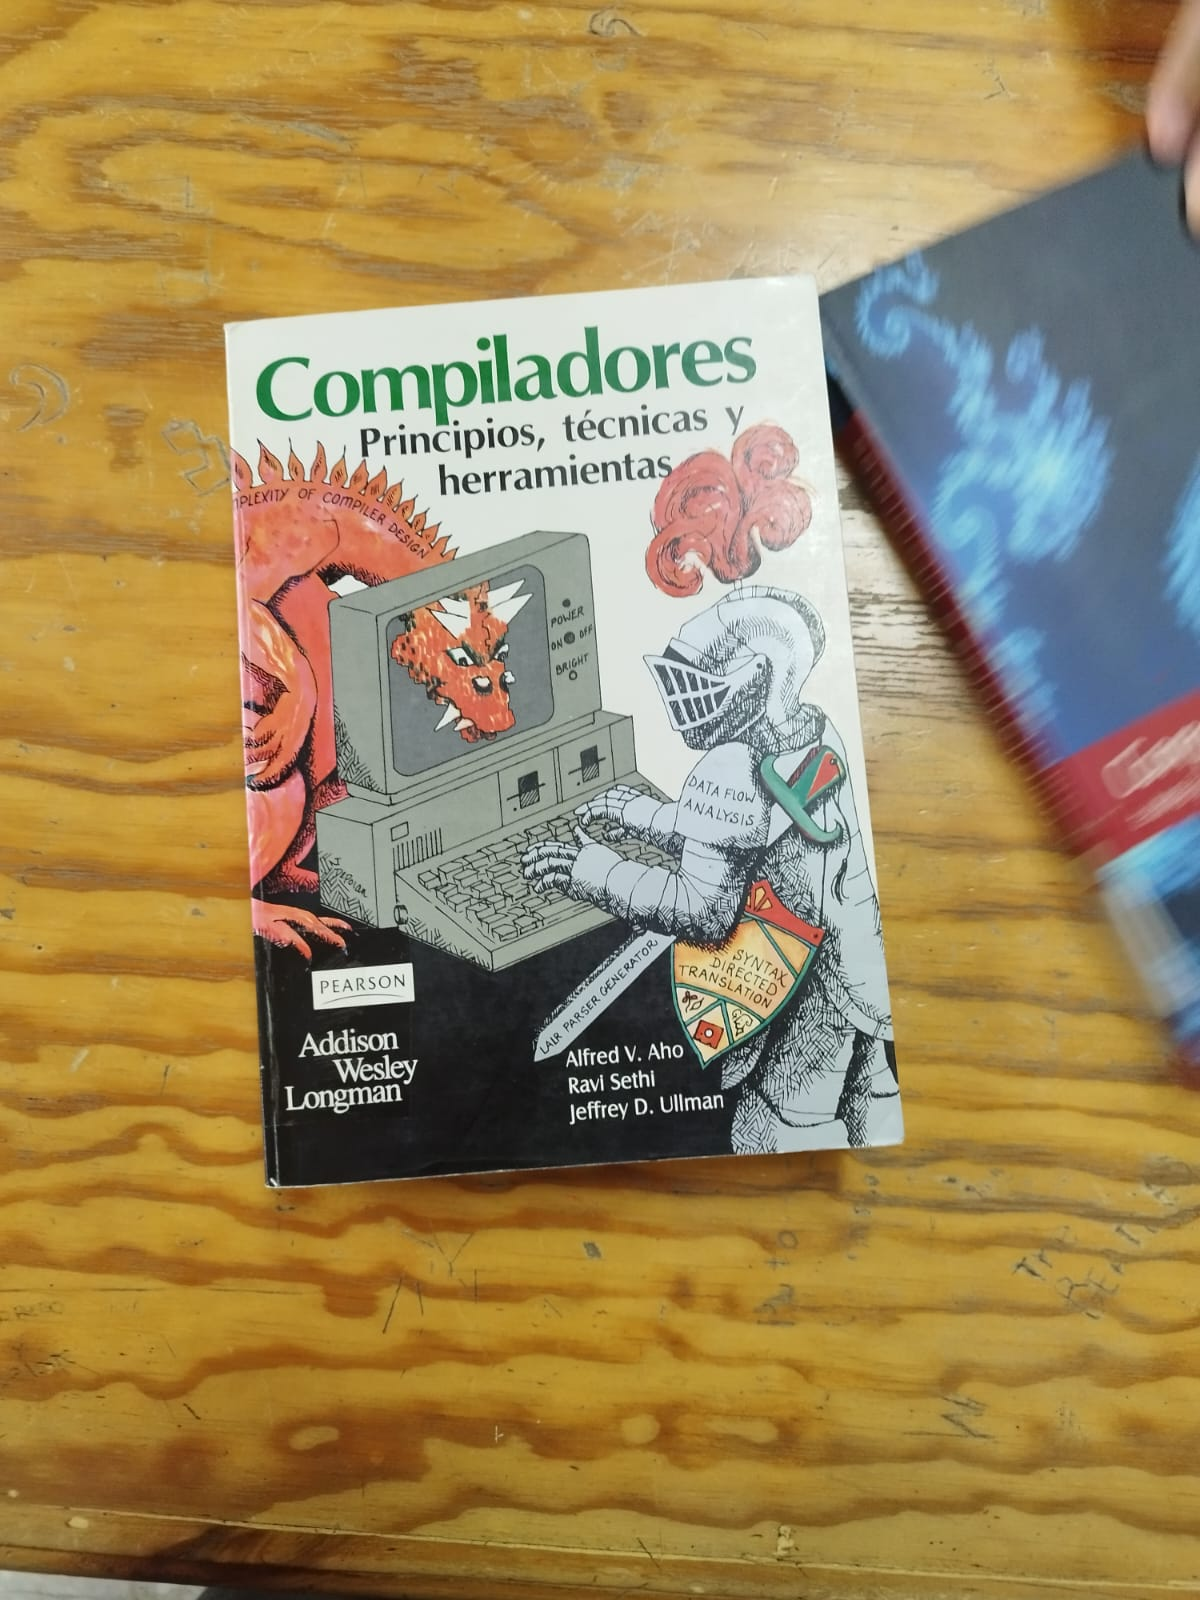
\includegraphics[width=0.9\linewidth]{imagenes/Imagen de WhatsApp 2025-10-17 a las 07.08.08_f83b5967.jpg}
  \end{minipage}
  \caption*{Imágenes adjuntas (WhatsApp)}
\end{figure}

\section{Referencias Bibliográficas}
    %Formato APA 7° Ed.
  \begin{thebibliography}{100}
    \bibitem{Codemath}
Codemath. (s.f.). \textit{Autómatas y Lenguajes Formales DESDE CERO} [Serie de videos]. YouTube. https://www.youtube.com/playlist?list=PLyRNgg3I27WiOZqDamrZon3QDPZMlZ5P4
  \end{thebibliography}

\end{document}
